\subsection{2d}
Map 2d is a representation of possible location of the agent.
\begin{figure}[H]
    \centering
    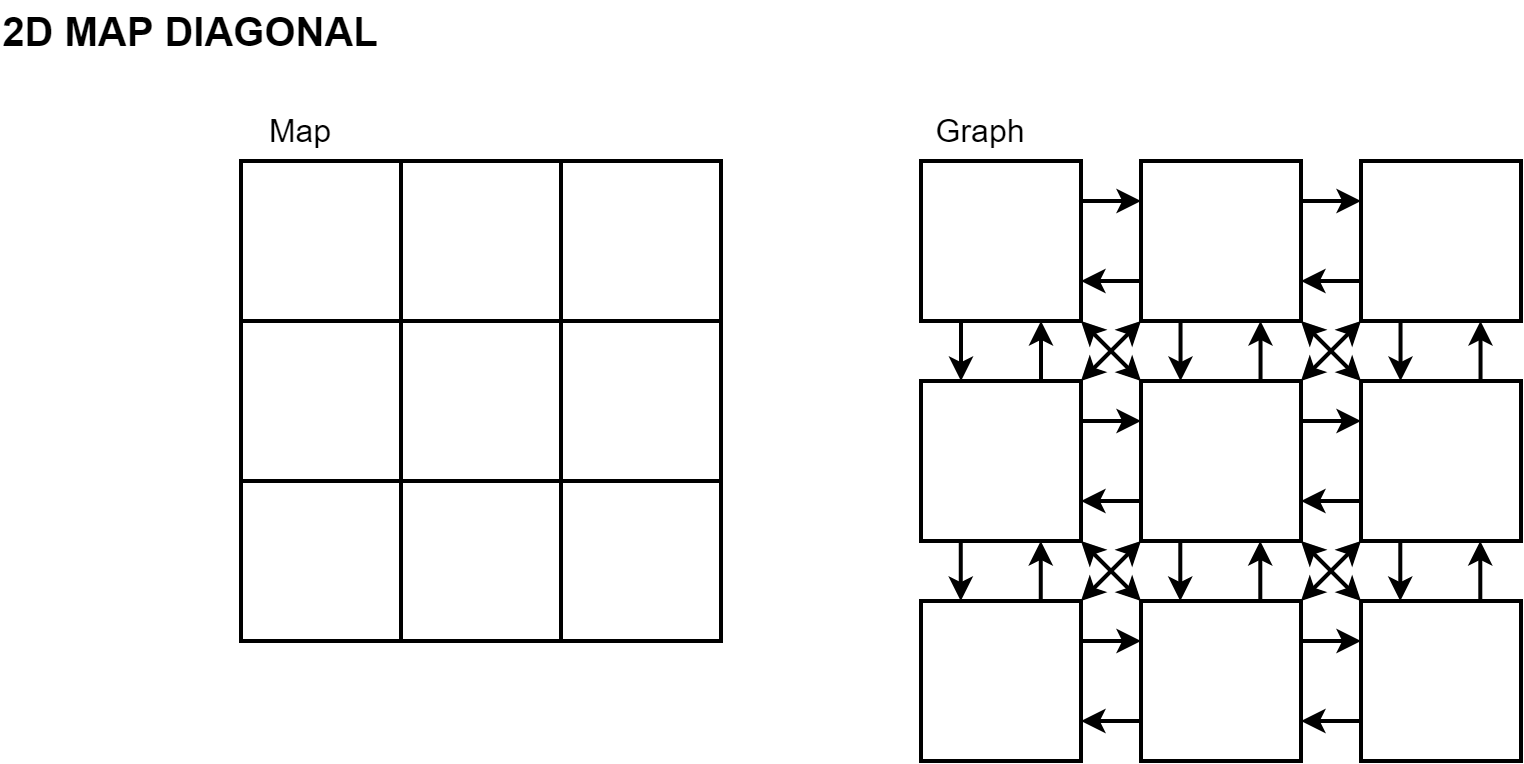
\includegraphics[width=0.8\textwidth]{pictures/map_2D_diag.png}
    \caption{ 2D map with diagonal movements allowed }
    \label{fig:map_2D_diag}
\end{figure}

\begin{figure}[H]
    \centering
    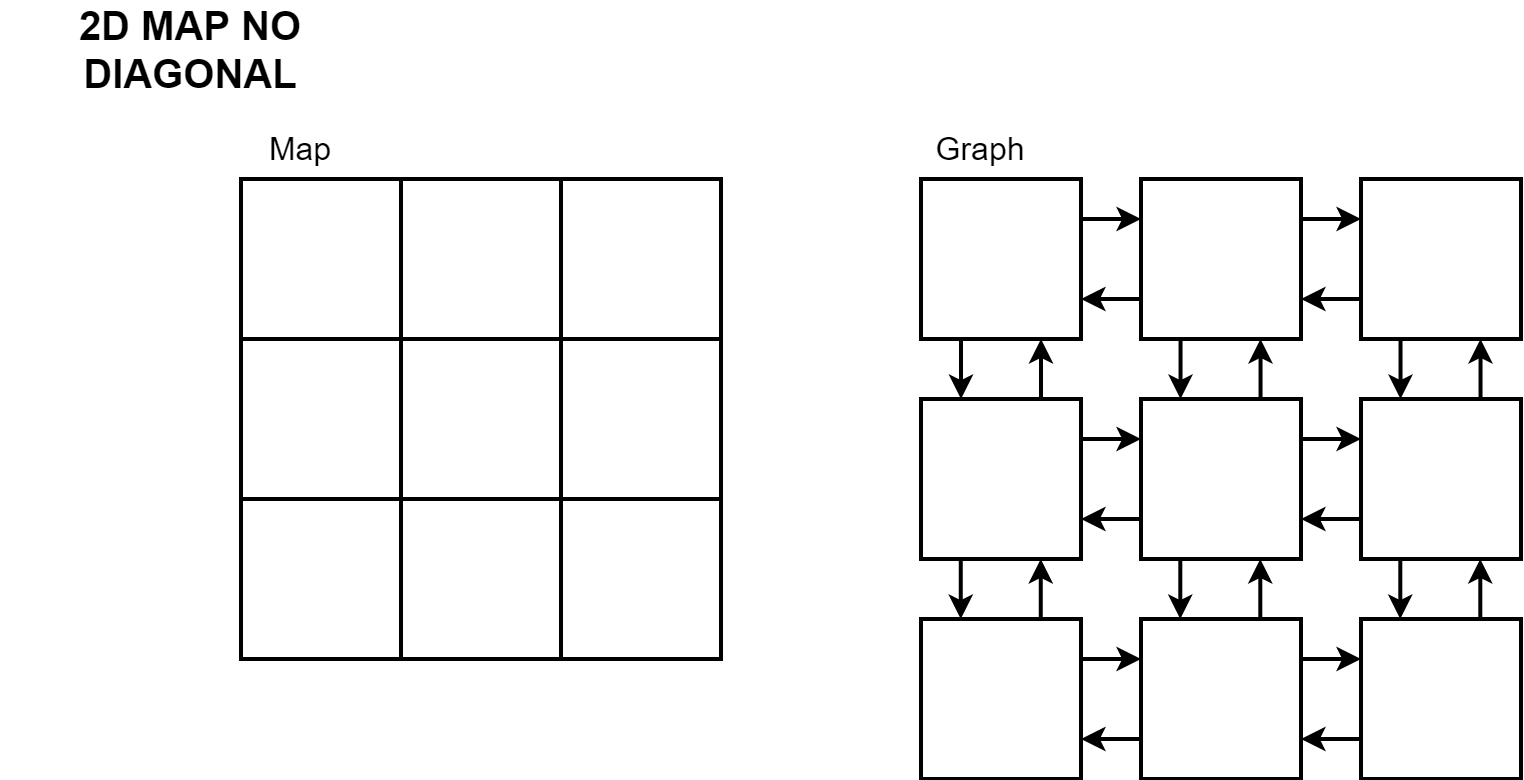
\includegraphics[width=0.8\textwidth]{pictures/map_2D_no_diag.png}
    \caption{ 3D map without diagonal movements allowed }
    \label{fig:map_2D_no_diag}
\end{figure}

\subsection{3d}
Map 2d is a representation of possible location of the agent with respect to the time which is represented as one of the dimensions in the map.
\begin{figure}[H]
    \centering
    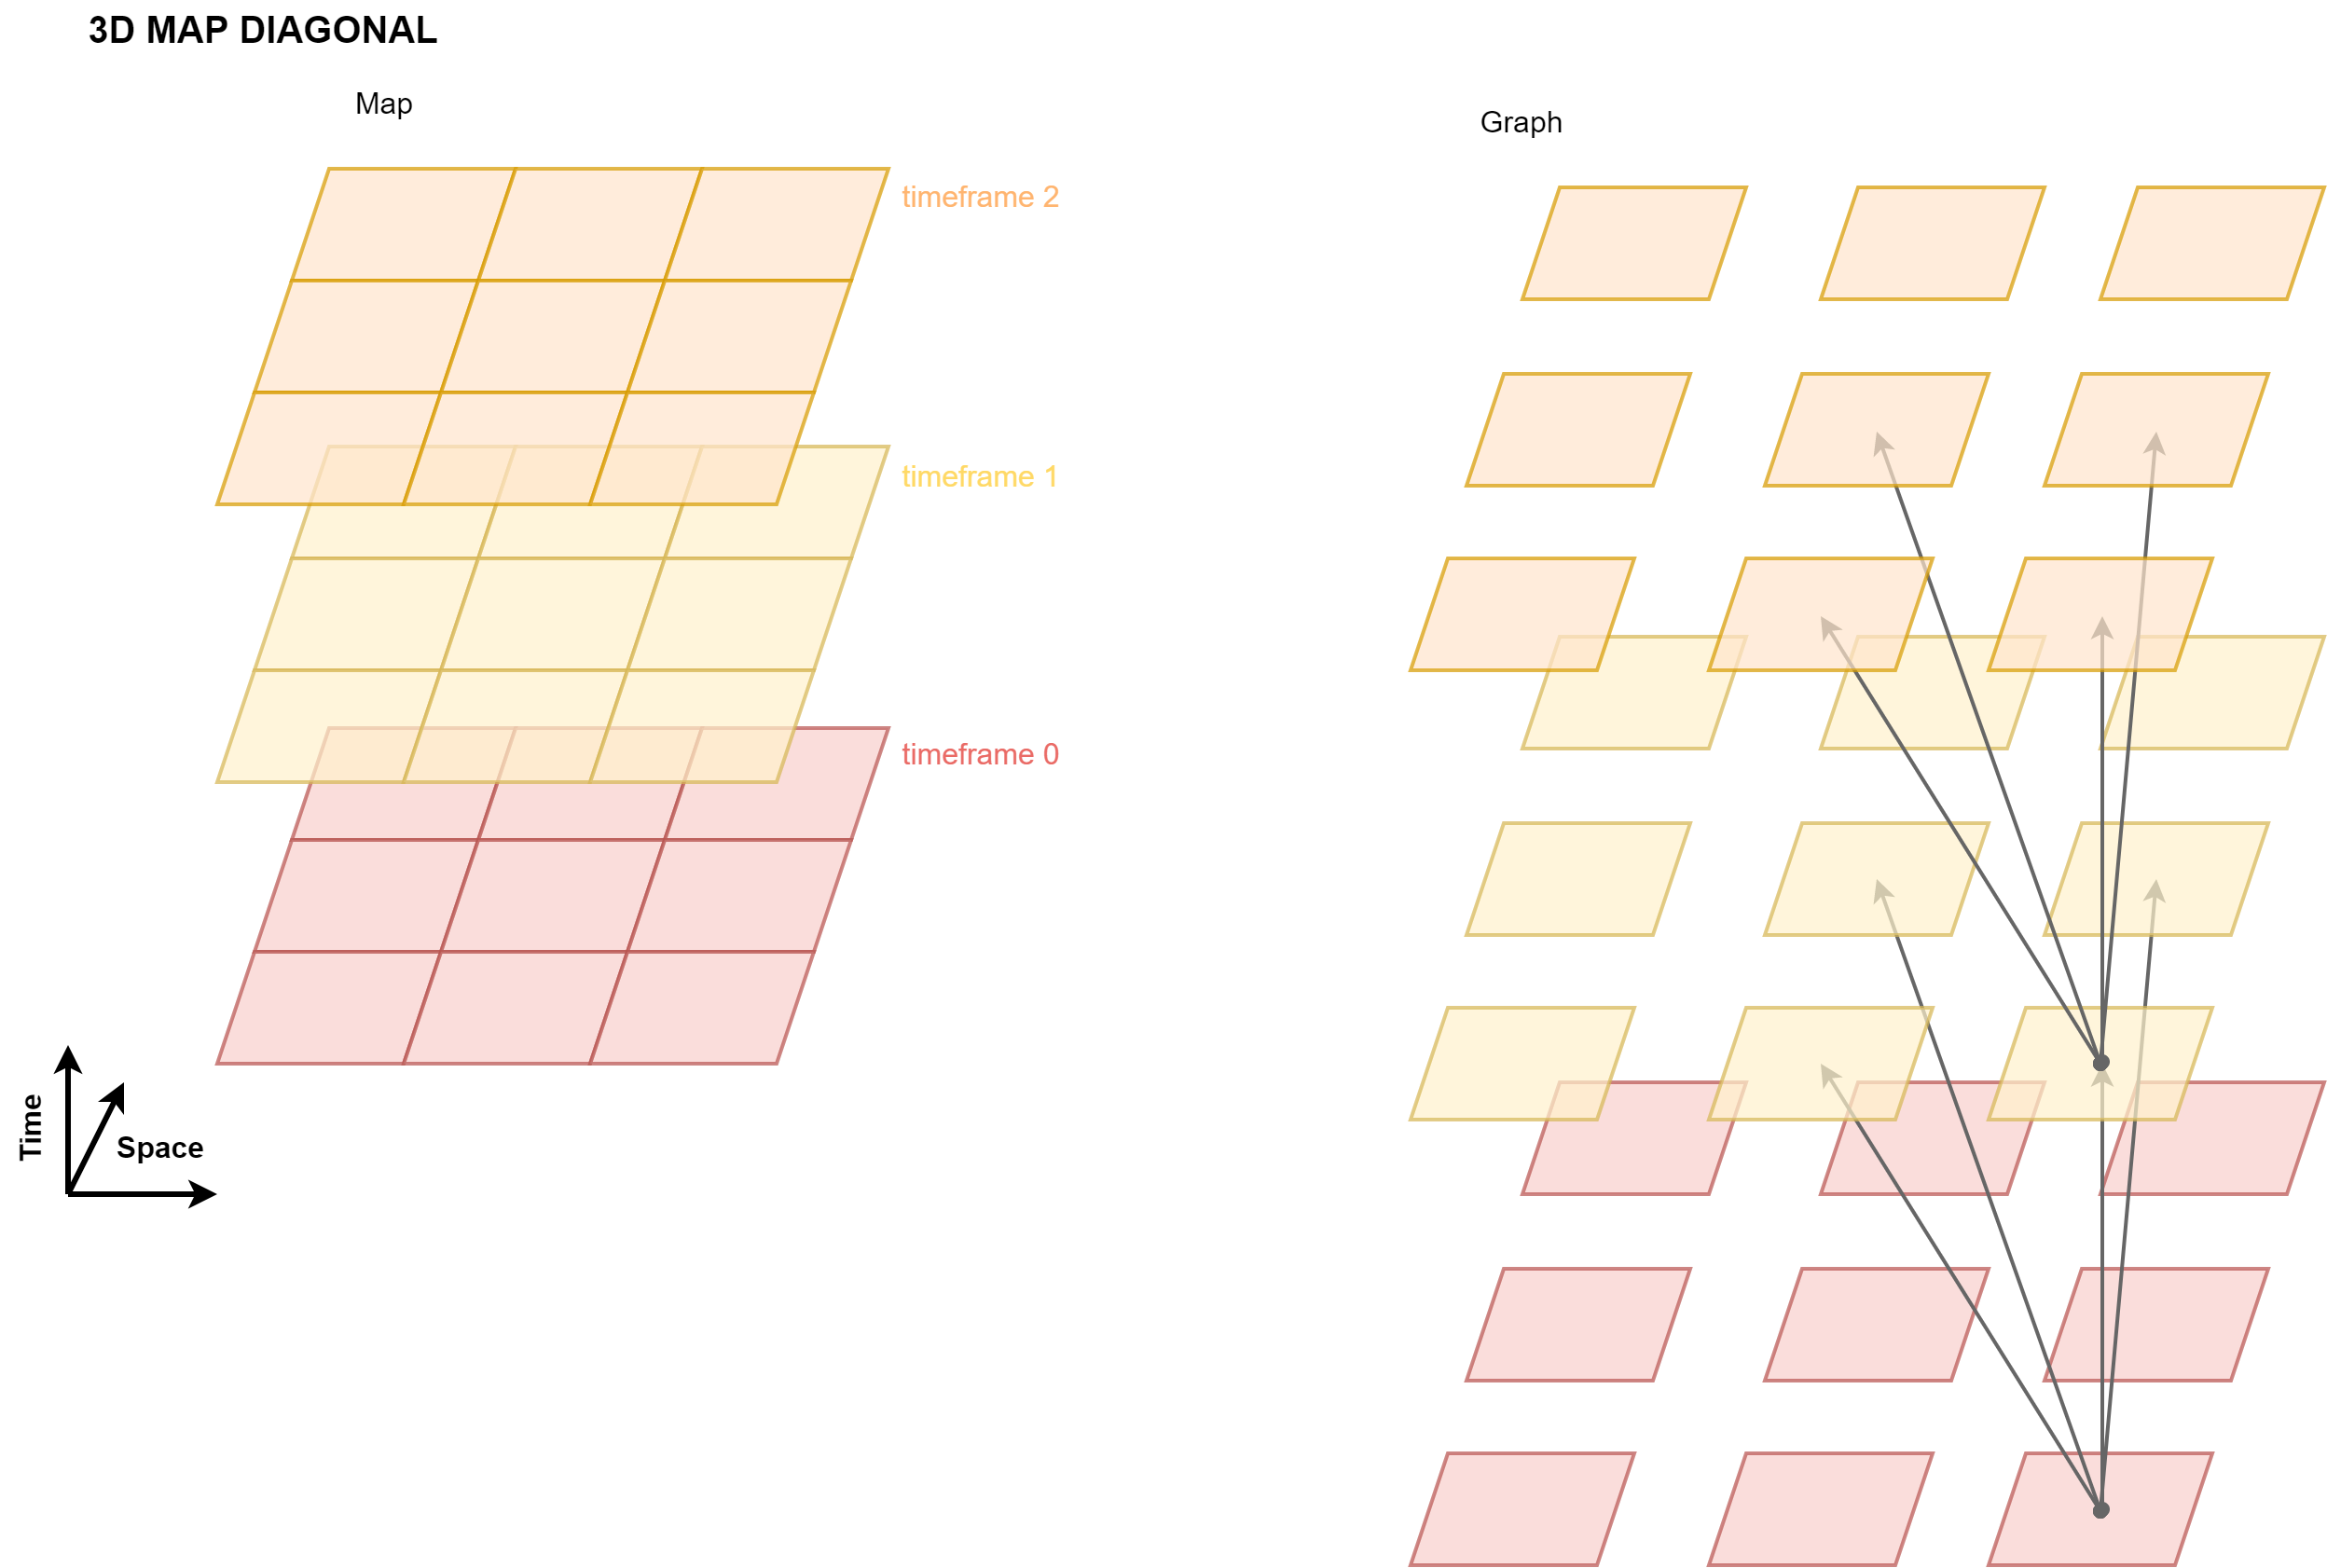
\includegraphics[width=0.8\textwidth]{pictures/map_3D_diag.png}
    \caption{ 3D map with diagonal movements allowed }
    \label{fig:map_3D_diag}
\end{figure}

\begin{figure}[H]
    \centering
    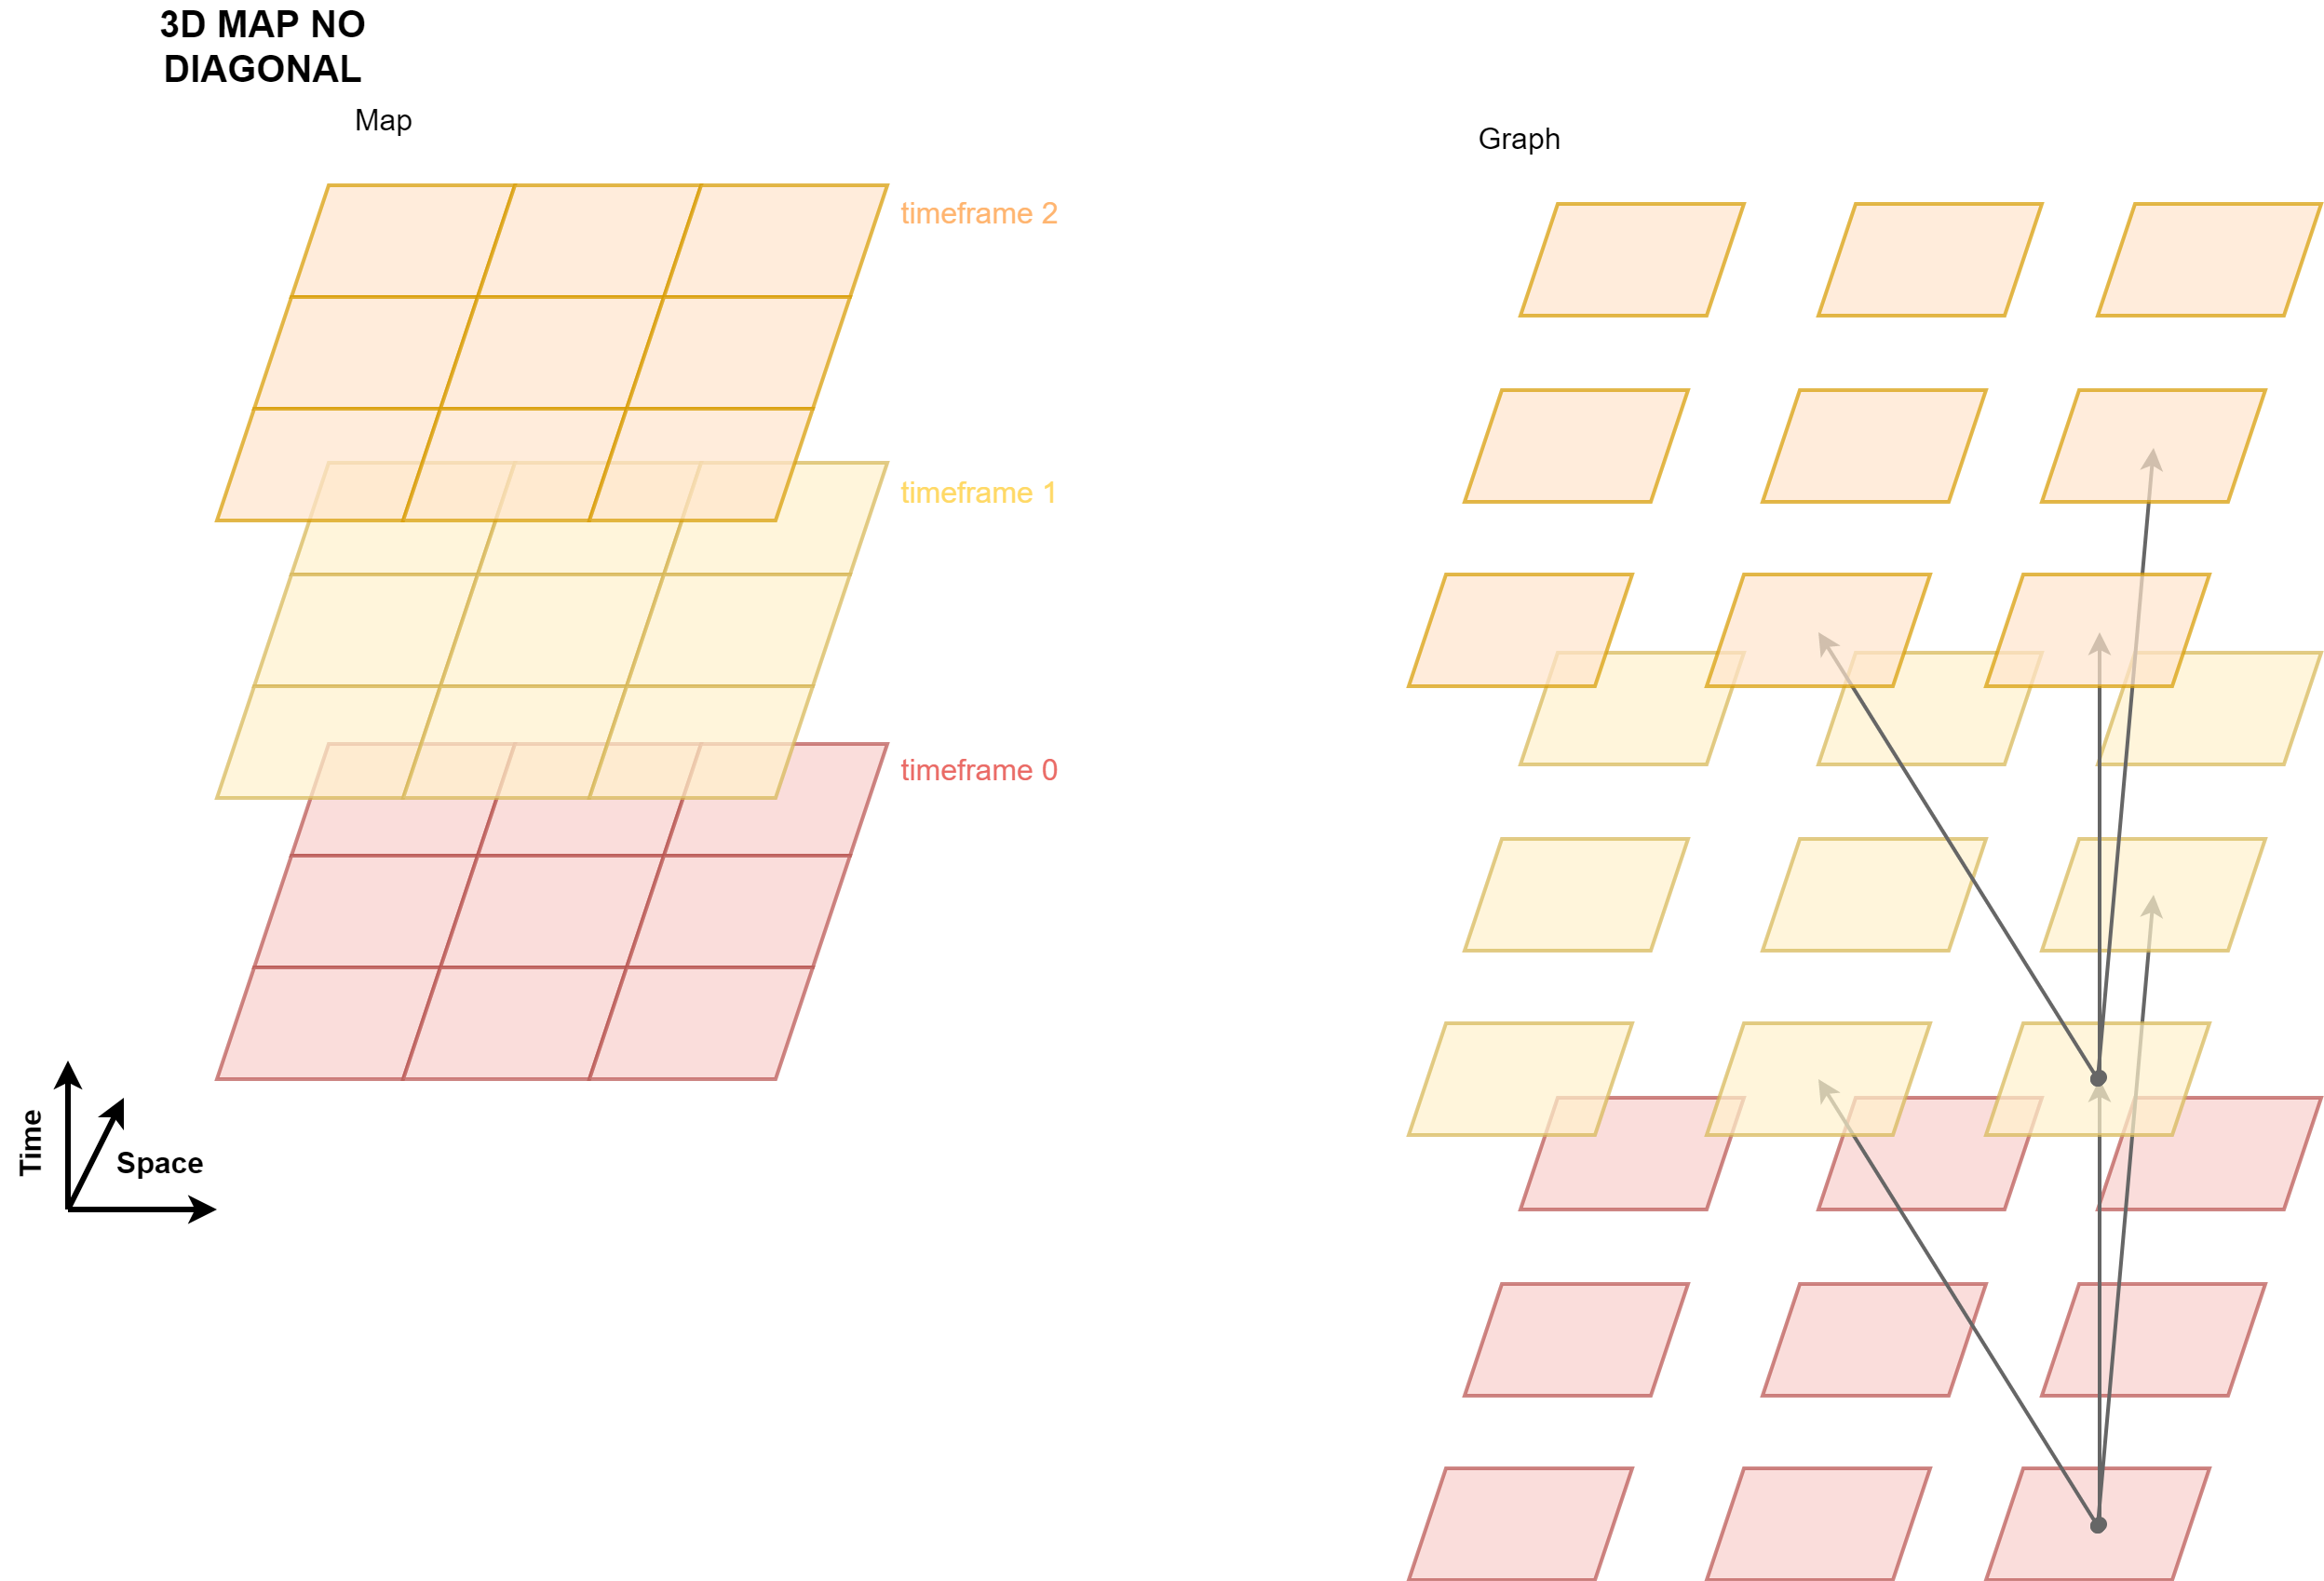
\includegraphics[width=0.8\textwidth]{pictures/map_3D_no_diag.png}
    \caption{ 3D map without diagonal movements allowed }
    \label{fig:map_3D_no_diag}
\end{figure}

\subsection{CA* front collision problem}

\begin{figure}[H]
    \centering
    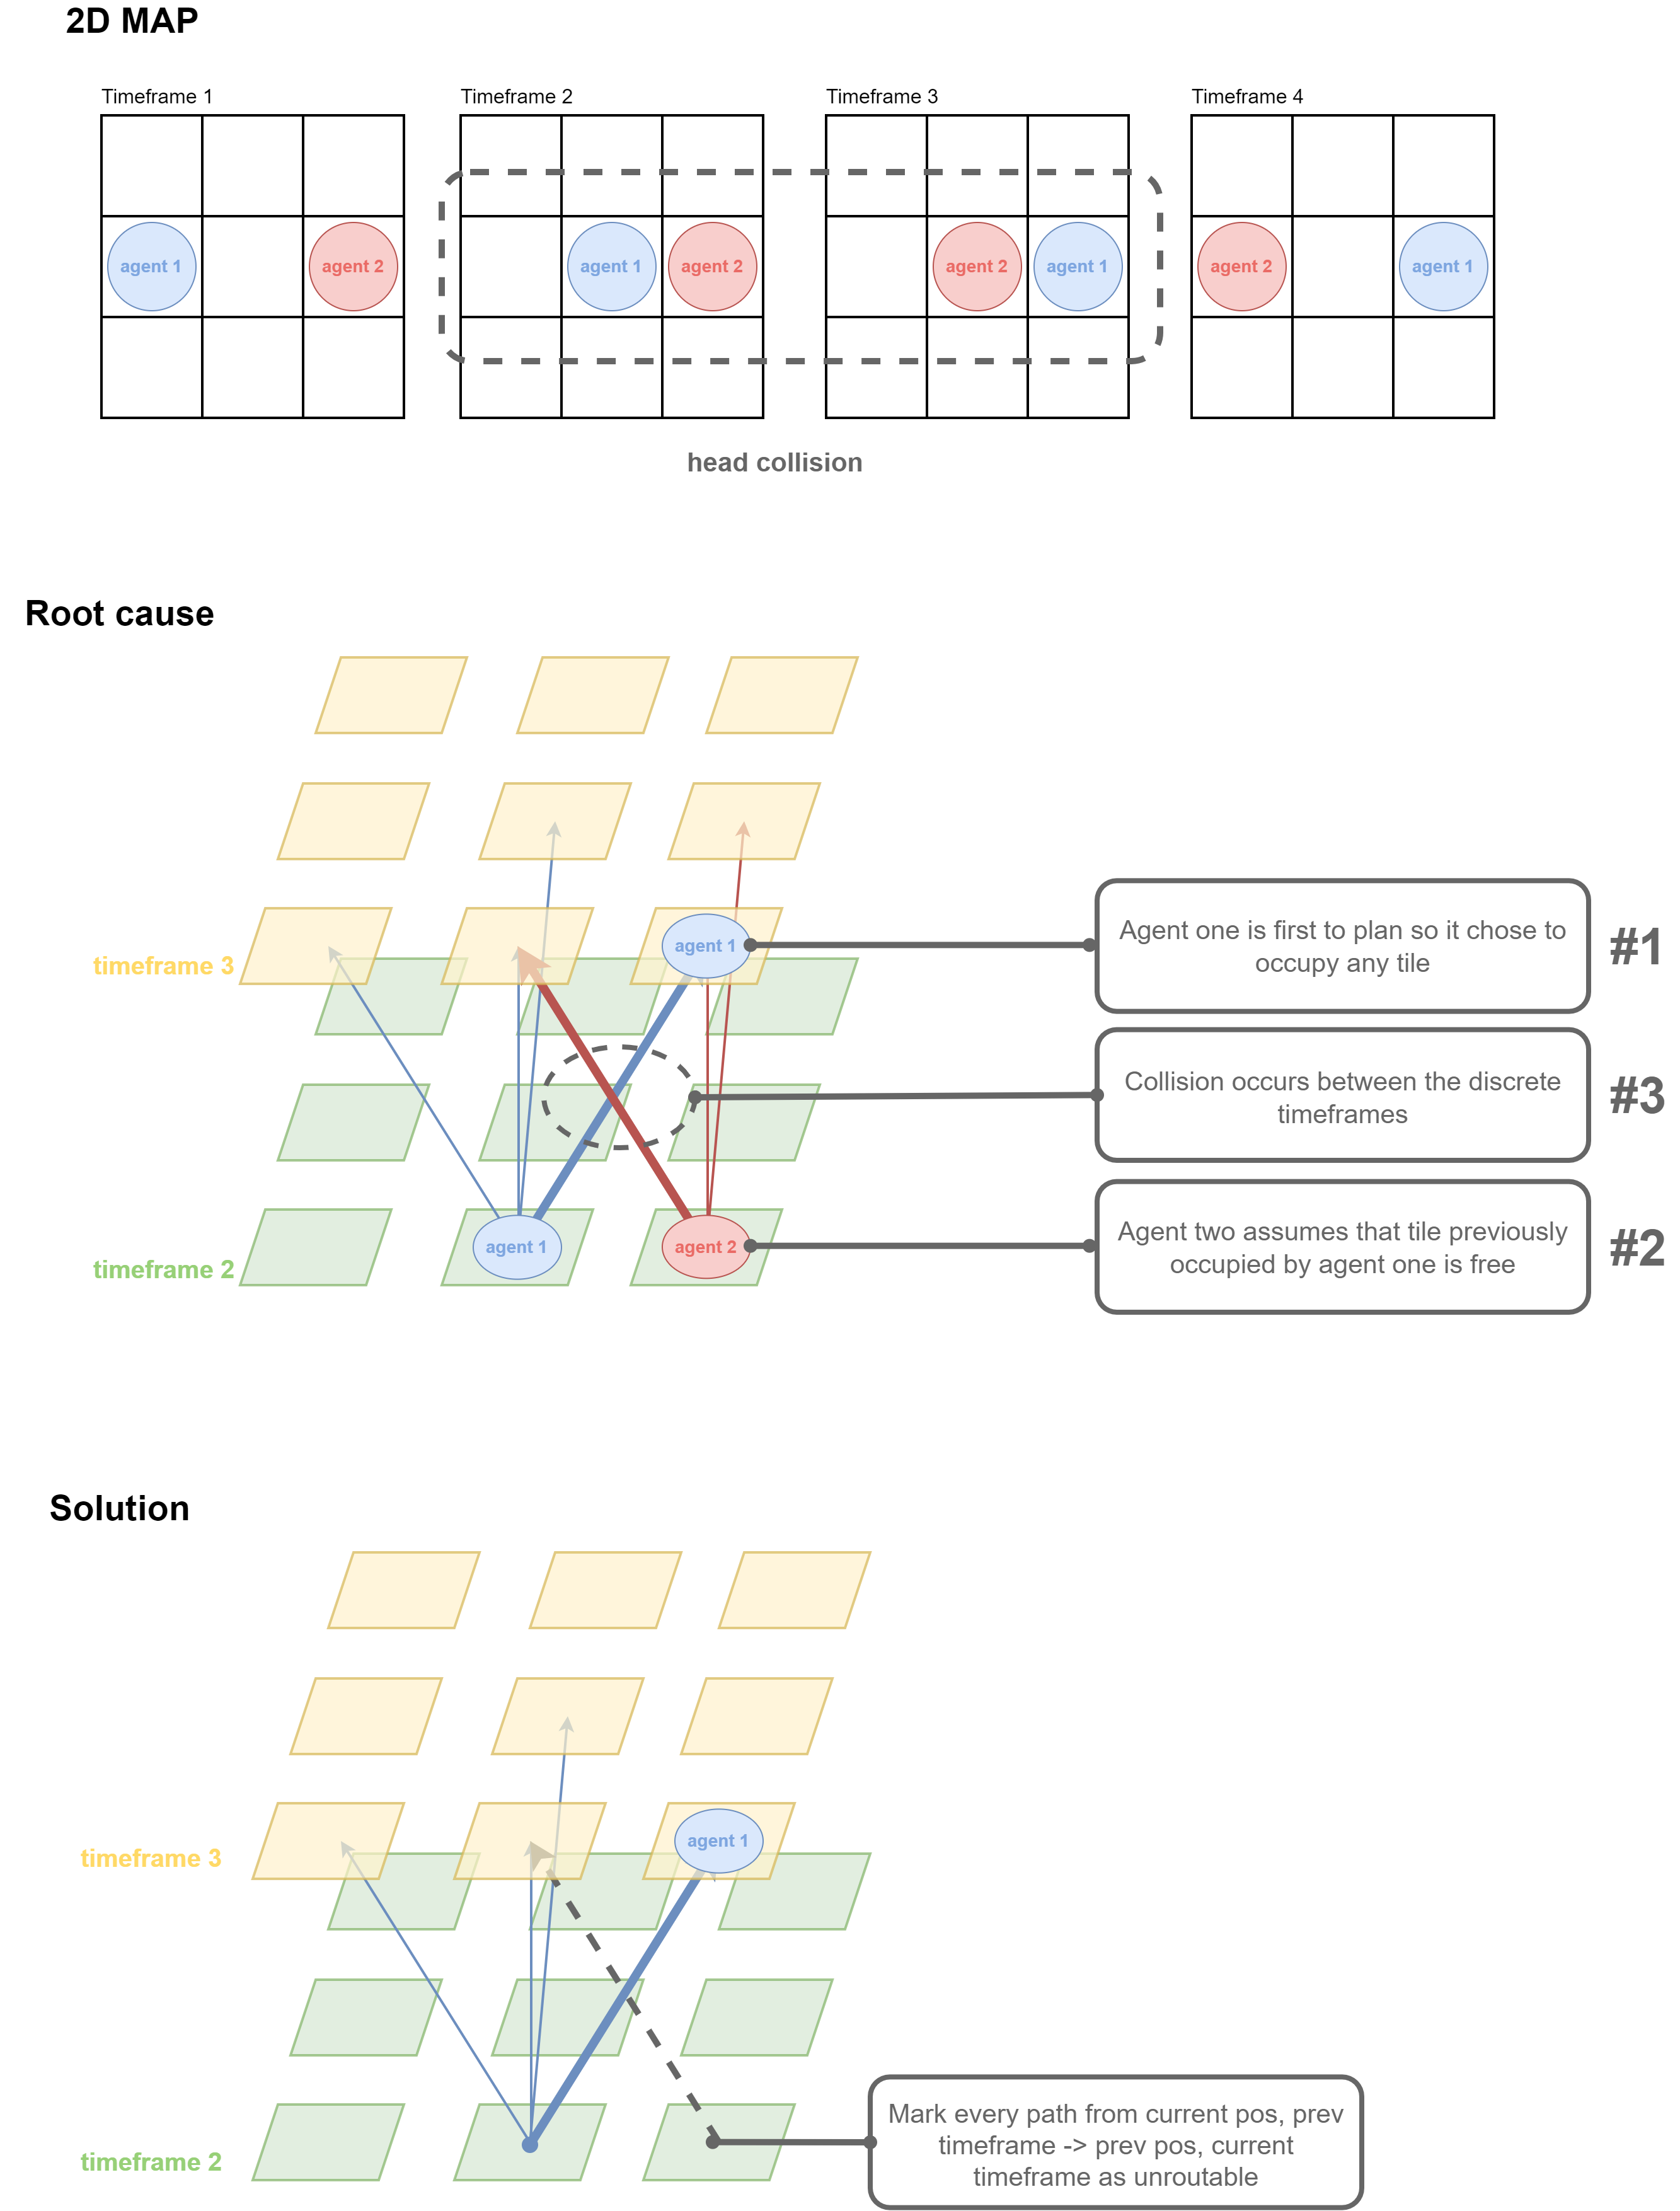
\includegraphics[width=0.8\textwidth]{pictures/head_collision_problem.png}
    \caption{ CA* head collision problem}
    \label{fig:head_collision}
\end{figure}